\documentclass[11pt]{article}
\usepackage{graphicx}
\usepackage{hyperref}
\usepackage{caption}
\usepackage{subcaption}

%numeroter les pages
\pagestyle{plain}

\usepackage[T1]{fontenc}
\usepackage[utf8]{inputenc}


\title{Modèle de Markov Caché pour la prise de décision de robots ou d'entités virtuelles}
\author{Arthur Le Guennec \and Kwon-Young Choi}
\date{\normalsize\today}
%%% END HEAD

\begin{document}
\maketitle

\section{Principe général des Modèles de Markov Caché}

Un HMM (Hidden Markov Model en anglais ou Modèle de Markov Caché en français) est une modélisation stochastique d’un automate avec des états cachés (notés Ht) et des états observables (notés St).
Les états cachés sont déterminés par un chaîne de Markov.
L'utilisation d'une chaine de Markov induit que le modèle est discret dans le temps et peut aussi être discret dans ses états.
Les chaine de Markov possède la propriété de Markov, ce qui implique que la probabilité d'être dans un état Ht+1 ne dépend pas de tous les états précédents.
Chacun des états du HMM a donc une probabilité de transition vers les autres états.
Les état observables ne dépendent donc que de l'état courant.

\begin{figure}[btp]
  \centering
  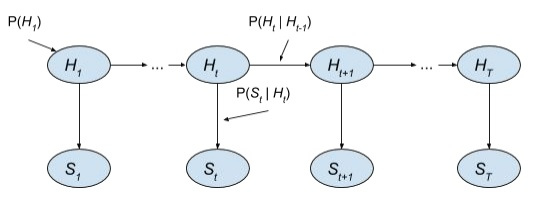
\includegraphics[scale=1]{hmm}
  \caption{\label{hmm} Modélisation d'un Modèle de Markov Caché.}
\end{figure}

Les HMM sont beaucoup utilisés dans  la reconnaissance de forme, comme la reconnaissance des gestes, ou la reconnaissance vocale.

\end{document}
